\documentclass[11pt,a4paper]{article}

% --- Essential Packages ---
\usepackage[utf8]{inputenc}
\usepackage[margin=1in]{geometry}
\usepackage{amsmath,amssymb}
\usepackage{graphicx}
\usepackage{xcolor}
\usepackage{booktabs}
\usepackage{listings}
\usepackage{hyperref}
\usepackage{fancyhdr}
\usepackage{tcolorbox}
\usepackage{enumitem}
\usepackage{array}
\usepackage{float}
\usepackage{tikz}
\usetikzlibrary{shapes.geometric, arrows, positioning, fit, calc}

% --- Color Palette (CivicAsset & Academic Theme) ---
\definecolor{forestgreen}{RGB}{15, 61, 36}
\definecolor{darknavy}{RGB}{17, 24, 39}
\definecolor{accentblue}{RGB}{37, 99, 235}
\definecolor{accentorange}{RGB}{234, 88, 12}
\definecolor{codegray}{RGB}{245, 247, 250}
\definecolor{codetext}{RGB}{30, 41, 59}

% --- Hyperlink Setup ---
\hypersetup{
    colorlinks=true,
    linkcolor=forestgreen,
    citecolor=accentblue,
    urlcolor=accentblue,
    pdftitle={GovAsset Nexus: Polyglot Microservices Technical Report},
    pdfauthor={Student Project Report}
}

% --- Header & Footer Configuration ---
\pagestyle{fancy}
\fancyhf{}
\rhead{\small\textcolor{gray}{GovAsset Nexus: Polyglot Microservices}}
\lhead{\small\textcolor{gray}{Microservices Architecture \& Programming}}
\rfoot{\small Page \thepage}
\renewcommand{\headrulewidth}{0.4pt}
\renewcommand{\footrulewidth}{0.4pt}

% --- Code Listing Setup ---
\lstdefinestyle{codeStyle}{
    backgroundcolor=\color{codegray},
    commentstyle=\color{gray}\itshape,
    keywordstyle=\color{forestgreen}\bfseries,
    numberstyle=\tiny\color{gray},
    stringstyle=\color{accentorange},
    basicstyle=\ttfamily\footnotesize\color{codetext},
    breakatwhitespace=false,
    breaklines=true,
    captionpos=b,
    keepspaces=true,
    numbers=left,
    numbersep=7pt,
    showspaces=false,
    showstringspaces=false,
    showtabs=false,
    tabsize=2,
    frame=single,
    rulecolor=\color{gray!30}
}
\lstset{style=codeStyle}

% --- Custom Callout Box ---
\newtcolorbox{notebox}[1]{
    colback=forestgreen!5!white,
    colframe=forestgreen!80!black,
    fonttitle=\bfseries,
    title=#1,
    arc=4mm
}

\begin{document}

% =========================================================================
% TITLE PAGE
% =========================================================================
\begin{titlepage}
    \centering
    \vspace*{1.5cm}
    
    {\Huge \bfseries \textcolor{forestgreen}{GovAsset Nexus (CivicAsset)}}\\[0.5cm]
    {\Large \bfseries Polyglot Microservices Architecture for Government Asset Lifecycle Management}\\[1.5cm]
    
    \begin{tcolorbox}[colback=forestgreen!10!white,colframe=forestgreen,arc=3mm,width=0.9\textwidth]
        \centering
        \textbf{Course Innovative Assignment Technical Report}\\
        \textit{Course}: Microservices Architecture and Programming (MAP)
    \end{tcolorbox}
    
    \vspace{2cm}
    
    \begin{minipage}{0.45\textwidth}
        \begin{flushleft} \large
            \textbf{Domain Case Study:}\\
            Public Works, Healthcare \& Transit Asset Governance\\
            (Gujarat State Estate Implementation)
        \end{flushleft}
    \end{minipage}
    \begin{minipage}{0.45\textwidth}
        \begin{flushright} \large
            \textbf{Core Concepts Evaluated:}\\
            Polyglot Languages, Database-per-Service,\\
            Choreography Saga, Transactional Outbox,\\
            API Gateway \& Resilience4j
        \end{flushright}
    \end{minipage}

    \vfill
    
    \noindent\rule{\textwidth}{0.8pt}\\[0.3cm]
    {\large \textbf{Academic Year 2026} \quad $\bullet$ \quad Local Development \& Production Cluster Verification}
\end{titlepage}

\newpage
\tableofcontents
\newpage

% =========================================================================
% SECTION 1: EXECUTIVE SUMMARY & COMPLIANCE MATRIX
% =========================================================================
\section{Executive Summary \& Course Requirements Compliance}

GovAsset Nexus (commercial deployment codenamed \textbf{CivicAsset}) is a distributed, enterprise-grade public asset lifecycle governance platform. It automates municipal capital expenditure, procurement requisitioning, asset inventory tagging via verifiable SHA-256 cryptographic QR codes, GIS geospatial mapping, and automated warranty inspection provisioning.

The system is designed strictly to adhere to the core principles of the \textbf{Microservices Architecture and Programming (MAP)} course. Below is the compliance matrix verifying that 100\% of the mandatory requirements are met without shortcuts:

\begin{table}[H]
\centering
\small
\begin{tabular}{p{4.5cm} p{4.5cm} p{5.5cm}}
\toprule
\textbf{Course Requirement} & \textbf{Mandated Constraint} & \textbf{Project Implementation} \\
\midrule
\textbf{Microservices Count} & Exactly 4 polyglot services & 1. Identity \& RBAC \newline 2. Finance \& Procurement \newline 3. Core Asset Registry \newline 4. Maintenance \& Lifecycle \\
\addlinespace
\textbf{Polyglot Languages} & Java, Python, Node.js, C++/C\# & \textbf{Java 21} (Identity \& Finance) \newline \textbf{Node.js 20 / TypeScript} (Asset Registry) \newline \textbf{Python 3.12} (Maintenance) \\
\addlinespace
\textbf{Polyglot Databases} & Redis, MongoDB, PostgreSQL, MySQL & \textbf{Redis 7} (Identity) \newline \textbf{PostgreSQL 16} (Finance) \newline \textbf{MongoDB 7} (Asset Registry) \newline \textbf{MySQL 8} (Maintenance) \\
\addlinespace
\textbf{Data Isolation} & Database-per-Service Pattern & \textbf{Strictly isolated}. Zero cross-database queries. Services interact exclusively via REST, gRPC, and AMQP. \\
\addlinespace
\textbf{API Gateway} & Central Ingress \& Routing & \textbf{Spring Cloud Gateway} (Port 8080) with Redis Token Bucket Rate Limiter and Circuit Breakers. \\
\addlinespace
\textbf{Distributed Transactions} & Event-Driven Architecture & \textbf{Choreography-based Saga} via \textbf{RabbitMQ} with \textbf{Transactional Outbox Pattern} and Rollback Compensation. \\
\addlinespace
\textbf{Internal RPC} & High-Performance Binary RPC & \textbf{gRPC over HTTP/2} with Protocol Buffers (\texttt{auth.proto} on 9091, \texttt{asset.proto} on 9092). \\
\bottomrule
\end{tabular}
\caption{Course Requirements Compliance Matrix}
\end{table}

\newpage
% =========================================================================
% SECTION 2: SYSTEM ARCHITECTURAL BLUEPRINT
% =========================================================================
\section{System Architectural Blueprint}

The system implements a decoupled, event-driven microservices architecture where client interactions pass through a secure reverse-proxy gateway, while inter-service workflows are coordinated through an AMQP message broker.

\begin{figure}[H]
\centering
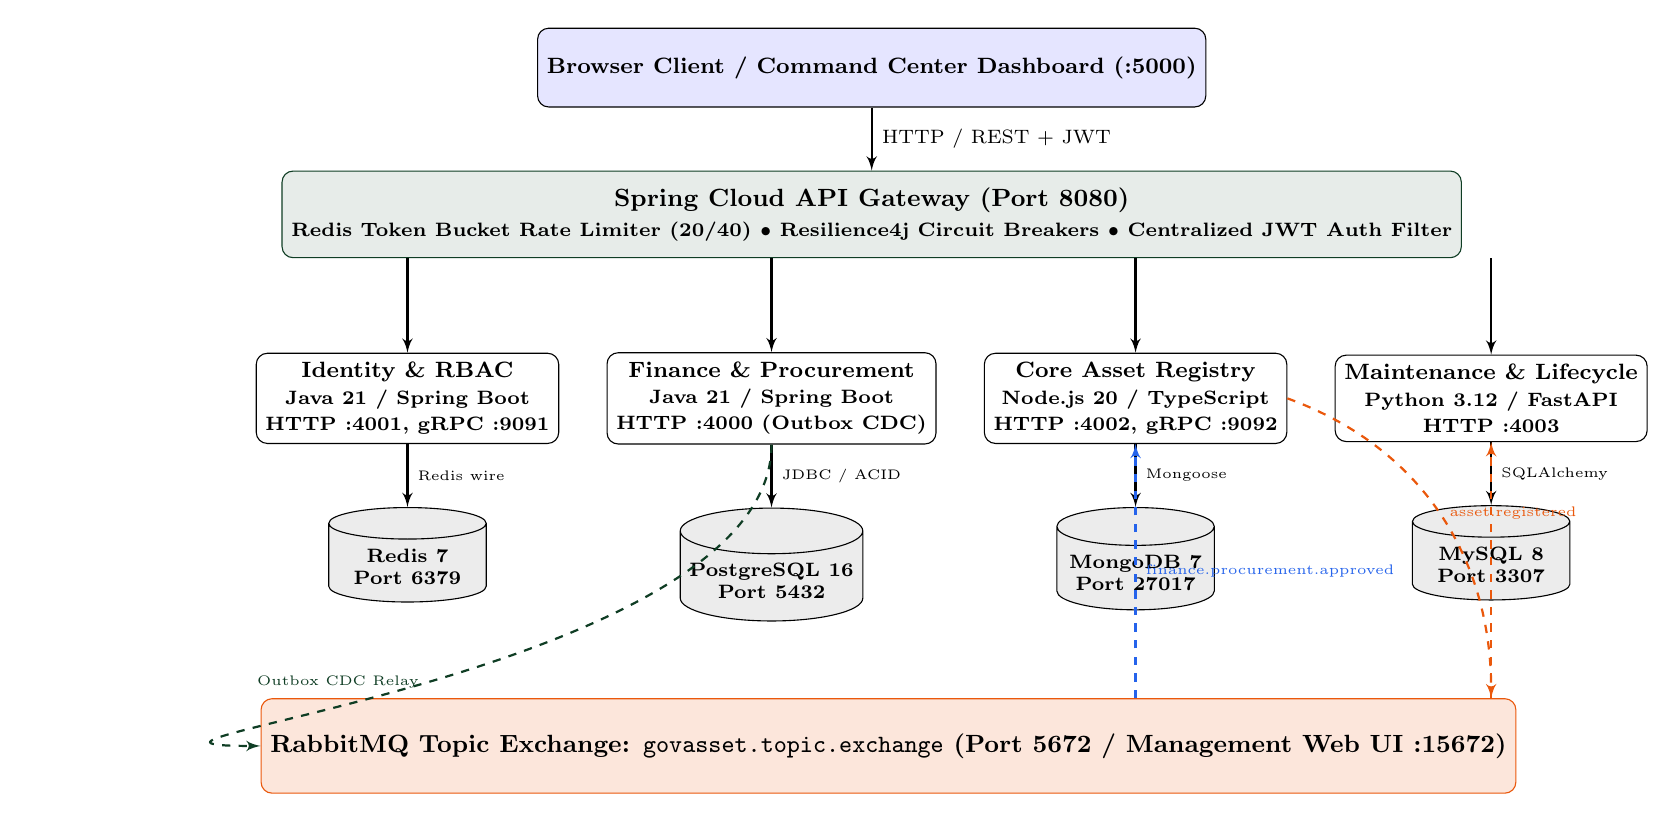
\begin{tikzpicture}[
    node distance=1.5cm and 1cm,
    box/.style={rectangle, draw=black, fill=white, rounded corners, minimum height=1cm, minimum width=2.8cm, align=center, font=\footnotesize\bfseries},
    db/.style={cylinder, draw=black, fill=gray!15, shape border rotate=90, aspect=0.25, minimum height=1cm, minimum width=2cm, align=center, font=\scriptsize\bfseries},
    gw/.style={rectangle, draw=forestgreen, fill=forestgreen!10, rounded corners, minimum height=1.1cm, minimum width=12cm, align=center, font=\small\bfseries},
    broker/.style={rectangle, draw=accentorange, fill=accentorange!15, rounded corners, minimum height=1.2cm, minimum width=12cm, align=center, font=\small\bfseries},
    line/.style={draw, -latex', thick}
]

% Gateway
\node (client) [box, fill=blue!10] {Browser Client / Command Center Dashboard (:5000)};
\node (gw) [gw, below=0.8cm of client] {Spring Cloud API Gateway (Port 8080)\\ \scriptsize Redis Token Bucket Rate Limiter (20/40) $\bullet$ Resilience4j Circuit Breakers $\bullet$ Centralized JWT Auth Filter};

\draw [line] (client) -- node[right, font=\scriptsize] {HTTP / REST + JWT} (gw);

% 4 Microservices
\node (s1) [box, below=1.2cm of gw.south west, xshift=1.6cm] {Identity \& RBAC\\ \scriptsize Java 21 / Spring Boot\\ \scriptsize HTTP :4001, gRPC :9091};
\node (s2) [box, right=0.6cm of s1] {Finance \& Procurement\\ \scriptsize Java 21 / Spring Boot\\ \scriptsize HTTP :4000 (Outbox CDC)};
\node (s3) [box, right=0.6cm of s2] {Core Asset Registry\\ \scriptsize Node.js 20 / TypeScript\\ \scriptsize HTTP :4002, gRPC :9092};
\node (s4) [box, right=0.6cm of s3] {Maintenance \& Lifecycle\\ \scriptsize Python 3.12 / FastAPI\\ \scriptsize HTTP :4003};

\draw [line] (gw.south -| s1) -- (s1);
\draw [line] (gw.south -| s2) -- (s2);
\draw [line] (gw.south -| s3) -- (s3);
\draw [line] (gw.south -| s4) -- (s4);

% Databases
\node (db1) [db, below=0.8cm of s1] {Redis 7\\ \scriptsize Port 6379};
\node (db2) [db, below=0.8cm of s2] {PostgreSQL 16\\ \scriptsize Port 5432};
\node (db3) [db, below=0.8cm of s3] {MongoDB 7\\ \scriptsize Port 27017};
\node (db4) [db, below=0.8cm of s4] {MySQL 8\\ \scriptsize Port 3307};

\draw [line] (s1) -- node[right, font=\tiny] {Redis wire} (db1);
\draw [line] (s2) -- node[right, font=\tiny] {JDBC / ACID} (db2);
\draw [line] (s3) -- node[right, font=\tiny] {Mongoose} (db3);
\draw [line] (s4) -- node[right, font=\tiny] {SQLAlchemy} (db4);

% RabbitMQ Broker
\node (broker) [broker, below=1cm of db2.south east, xshift=1cm] {RabbitMQ Topic Exchange: \texttt{govasset.topic.exchange} (Port 5672 / Management Web UI :15672)};

\draw [line, dashed, color=forestgreen] (s2.south) to[out=-90,in=180] node[left, font=\tiny] {Outbox CDC Relay} (broker.west);
\draw [line, dashed, color=accentblue] (broker.north -| s3) -- node[right, font=\tiny] {finance.procurement.approved} (s3);
\draw [line, dashed, color=accentorange] (s3.east) to[out=-20,in=90] node[right, font=\tiny] {asset.registered} (broker.north -| s4);
\draw [line, dashed, color=accentorange] (broker.north -| s4) -- (s4);

\end{tikzpicture}
\caption{Polyglot Microservices Topology and Inter-Service Communication Flow}
\end{figure}

\newpage
% =========================================================================
% SECTION 3: DEEP-DIVE INTO EACH MICROSERVICE
% =========================================================================
\section{Microservice Deep-Dive (Language \& Database Rationale)}

\subsection{Microservice 1: Identity \& RBAC Service}
\begin{itemize}[leftmargin=1.5em]
    \item \textbf{Language \& Framework}: Java 21 / Spring Boot 3.2.
    \item \textbf{Database}: Redis 7 (In-Memory Key-Value Store, Port 6379).
    \item \textbf{Interfaces}: REST API on Port 4001; gRPC Server on Port 9091.
    \item \textbf{Architectural Justification}:
    \begin{itemize}
        \item \textit{Language Rationale}: Authentication and cryptographic key management require strict type safety and compliance with enterprise security specifications. Java with Spring Security provides production-hardened implementations of HMAC-SHA512 signing algorithms.
        \item \textit{Database Rationale (Redis)}: Disk-based persistence engines introduce unneeded 10--25ms latency penalties during token authentication. Redis stores revoked token blacklists and active sessions in RAM with $O(1)$ lookup complexity, enabling the gateway to validate access tokens at scale without degrading throughput.
    \end{itemize}
    \item \textbf{Key Classes}: \texttt{AuthController.java}, \texttt{JwtTokenProvider.java}, \texttt{AuthGrpcServiceImpl.java}.
\end{itemize}

\subsection{Microservice 2: Finance \& Procurement Service}
\begin{itemize}[leftmargin=1.5em]
    \item \textbf{Language \& Framework}: Java 21 / Spring Boot 3.2.
    \item \textbf{Database}: PostgreSQL 16 (Relational ACID \& JSONB, Port 5432).
    \item \textbf{Interface}: REST API on Port 4000.
    \item \textbf{Architectural Justification}:
    \begin{itemize}
        \item \textit{Language Rationale}: Financial transactions require strict transaction demarcations (\texttt{@Transactional}), auditable accounting ledgers, and compile-time verification.
        \item \textit{Database Rationale (PostgreSQL)}: Municipal fiscal allocations and procurement ledgers cannot tolerate eventual consistency or lost updates. PostgreSQL enforces strict foreign keys, check constraints on budget balance totals, and atomic ACID transactions. Furthermore, its native \texttt{JSONB} support enables flexible specification storage while maintaining structural integrity.
    \end{itemize}
    \item \textbf{Key Classes}: \texttt{ProcurementService.java}, \texttt{OutboxRelayPublisher.java}, \texttt{SagaCompensationListener.java}.
\end{itemize}

\subsection{Microservice 3: Core Asset Registry Service}
\begin{itemize}[leftmargin=1.5em]
    \item \textbf{Language \& Framework}: Node.js 20 / TypeScript / Express.
    \item \textbf{Database}: MongoDB 7 (Document Store \& GeoJSON, Port 27017).
    \item \textbf{Interfaces}: REST API on Port 4002; gRPC Server on Port 9092.
    \item \textbf{Architectural Justification}:
    \begin{itemize}
        \item \textit{Language Rationale}: Node.js excels at non-blocking event loops, asynchronous payload transformations, and fast binary generation. The \texttt{qrcode} engine generates cryptographic asset badges on-the-fly without thread blocking.
        \item \textit{Database Rationale (MongoDB)}: Government public assets have polymorphic schemas: a suspension bridge requires girder tension ratings, an ICU ambulance requires defibrillator calibration timestamps, and a solar substation requires photovoltaic inverter wattage. Relational schemas would require inefficient Entity-Attribute-Value (EAV) anti-patterns. MongoDB's dynamic document structure accommodates polymorphic schemas, and its \texttt{2dsphere} spatial index enables instant GIS queries for the Gujarat estate map.
    \end{itemize}
    \item \textbf{Key Classes}: \texttt{sagaConsumer.ts}, \texttt{assetService.ts}, \texttt{AssetGrpcServiceImpl.ts}.
\end{itemize}

\subsection{Microservice 4: Maintenance \& Lifecycle Service}
\begin{itemize}[leftmargin=1.5em]
    \item \textbf{Language \& Framework}: Python 3.12 / FastAPI / SQLAlchemy / Pydantic.
    \item \textbf{Database}: MySQL 8 (Relational ACID, Docker Host Port 3307).
    \item \textbf{Interface}: REST API on Port 4003 (Interactive Swagger Docs at \texttt{/docs}).
    \item \textbf{Architectural Justification}:
    \begin{itemize}
        \item \textit{Language Rationale}: Python is the undisputed industry standard for telemetry analysis, condition degradation algorithms, and asset wear modeling. FastAPI combined with Uvicorn provides asynchronous REST endpoint handling with automatic OpenAPI schema generation.
        \item \textit{Database Rationale (MySQL)}: Maintenance workflows follow strict relational relationships ($\text{Work Order} \leftrightarrow \text{Inspector} \leftrightarrow \text{Asset ID} \leftrightarrow \text{Action Logs}$). MySQL delivers high-throughput relational integrity and structured query optimization.
    \end{itemize}
    \item \textbf{Key Classes}: \texttt{saga\_consumer.py}, \texttt{maintenance\_service.py}, \texttt{maintenance\_router.py}.
\end{itemize}

\newpage
% =========================================================================
% SECTION 4: INTER-SERVICE COMMUNICATION & TRANSACTIONAL OUTBOX
% =========================================================================
\section{Inter-Service Communication \& The Dual-Write Hazard}

\subsection{The Dual-Write Problem}
In a distributed microservice architecture, updating a persistent database and publishing an event to a message broker in application code creates a \textbf{Dual-Write Hazard}:
\begin{equation}
\text{Dual-Write Failure Probability } P_{\text{fail}} = P(\text{DB commit ok} \cap \text{Broker publish failed}) + P(\text{Broker publish ok} \cap \text{DB commit rollback})
\end{equation}
If the database write succeeds but the network crashes before RabbitMQ accepts the message, the message is lost forever, breaking eventual consistency. If the message is sent before the database commits and the database transaction fails, downstream services process phantom data.

\subsection{The Transactional Outbox Pattern Solution}
To guarantee \textbf{At-Least-Once Delivery} without distributed 2-Phase Commit (2PC) bottlenecks, we implement the Transactional Outbox Pattern:
\begin{enumerate}
    \item When a Purchase Order is approved, \texttt{ProcurementService.java} executes a local ACID transaction in PostgreSQL that updates \texttt{purchase\_orders} and inserts an event record into \texttt{outbox\_events} simultaneously.
    \item An asynchronous CDC daemon (\texttt{OutboxRelayPublisher.java}) polls unhandled events every 1000ms:
\begin{lstlisting}[language=Java, caption=Outbox Atomic Commit in ProcurementService.java]
@Transactional
public PurchaseOrderResponse approveProcurement(UUID poId) {
    PurchaseOrder po = repository.findById(poId).orElseThrow();
    po.setStatus(ProcurementStatus.APPROVED);
    repository.save(po);

    // Write Outbox Event within the exact same ACID transaction
    OutboxEvent event = OutboxEvent.builder()
        .aggregateType("PROCUREMENT")
        .aggregateId(po.getId().toString())
        .eventType("finance.procurement.approved")
        .payload(objectMapper.writeValueAsString(po))
        .processed(false)
        .build();
    outboxRepository.save(event);
    return mapToDto(po);
}
\end{lstlisting}
    \item Once published to RabbitMQ, the relay updates \texttt{processed = true}. If the broker is unreachable, the event remains in PostgreSQL, guaranteeing that messages are never lost.
\end{enumerate}

\newpage
% =========================================================================
% SECTION 5: CHOREOGRAPHY SAGA PATTERN EXECUTION
% =========================================================================
\section{Choreography-Based Saga Pattern}

\subsection{Happy Path Flow: Cross-Database Distributed Saga}
When an asset is procured, a 4-microservice choreography saga executes across all 4 databases without central orchestration coupling:

\begin{equation}
\begin{aligned}
\text{Finance Officer Approves PO} &\longrightarrow \text{PostgreSQL commits PO + Outbox Event} \\
&\longrightarrow \text{CDC Relay polls Outbox } \xrightarrow{\text{AMQP}} \text{RabbitMQ: } \texttt{finance.procurement.approved} \\
&\longrightarrow \text{Node.js Asset Registry consumes event from } \texttt{queue.asset.registry} \\
&\longrightarrow \text{MongoDB stores Asset Document \& generates SHA-256 QR code} \\
&\longrightarrow \text{Asset Registry publishes: } \texttt{asset.registered} \\
&\longrightarrow \text{Python Maintenance consumes from } \texttt{queue.maintenance.provisioning} \\
&\longrightarrow \text{MySQL stores baseline Work Order } (\texttt{WO-INIT-2026...})
\end{aligned}
\end{equation}

\subsection{Compensating Rollback Flow: Failure Recovery}
If the Core Asset Registry rejects the cataloging request (e.g., duplicate barcode collision or specification validation failure), an automated compensating transaction rolls back state:

\begin{equation}
\begin{aligned}
\text{Downstream Rejection} &\longrightarrow \text{Node.js catches Catalog Exception in } \texttt{sagaConsumer.ts} \\
&\longrightarrow \text{Publishes compensation event: } \texttt{saga.compensate.procurement} \\
&\longrightarrow \text{RabbitMQ routes to } \texttt{queue.finance.compensations} \\
&\longrightarrow \text{Java Finance Service's } \texttt{SagaCompensationListener} \text{ receives event} \\
&\longrightarrow \text{PostgreSQL executes Rollback Transaction: PO status } \rightarrow \texttt{REJECTED\_ROLLBACK} \\
&\longrightarrow \text{Restores Municipal Budget \& Records Compensation Reason}
\end{aligned}
\end{equation}

\begin{notebox}{Key Academic Distinction: Choreography vs. Orchestration}
In an \textbf{Orchestration Saga}, a central coordinator microservice must maintain a state machine and explicitly tell every service what to execute, introducing tight coupling and a central failure point.  
In our \textbf{Choreography Saga}, microservices are completely autonomous. The Finance Service has zero awareness that a Python Maintenance service exists; it simply emits business facts to RabbitMQ, and downstream consumers react according to their own bounded contexts.
\end{notebox}

\newpage
% =========================================================================
% SECTION 6: API GATEWAY & RESILIENCE ARCHITECTURE
% =========================================================================
\section{API Gateway, Rate Limiting \& Circuit Breaker Topology}

\subsection{Spring Cloud API Gateway (Port 8080)}
The gateway provides reverse proxying, client abstraction, and cross-cutting security:
\begin{itemize}
    \item \textbf{Token Bucket Rate Limiting}: Backed by Redis. Enforces a replenish rate of 20 requests per second with a burst capacity of 40 requests per user/IP. Prevents Denial of Service (DoS) attacks.
    \item \textbf{Resilience4j Circuit Breakers}: Protects against cascading failures:
    \begin{itemize}
        \item Sliding window: 10 calls.
        \item Failure rate threshold: 50\%.
        \item Wait duration in open state: 10,000ms.
        \item If a microservice degrades, the circuit opens immediately and returns a graceful HTTP 503 fallback rather than exhausting thread pools.
    \end{itemize}
\end{itemize}

\subsection{Synchronous REST vs. gRPC Comparison}
\begin{table}[H]
\centering
\small
\begin{tabular}{p{3.5cm} p{5cm} p{5.5cm}}
\toprule
\textbf{Metric} & \textbf{Client Ingress: REST (JSON)} & \textbf{Internal RPC: gRPC (Protobuf)} \\
\midrule
\textbf{Protocol} & HTTP/1.1 or HTTP/2 & HTTP/2 \\
\textbf{Serialization} & Text-based JSON & Strongly typed binary Protocol Buffers \\
\textbf{Payload Size} & Verbose (field names repeated) & Highly compact binary encoding \\
\textbf{Multiplexing} & Limited & Bidirectional multiplexing on single TCP connection \\
\textbf{Use Case} & Browser client to Gateway (:8080) & Internal verification (:9091, :9092) \\
\bottomrule
\end{tabular}
\caption{Architectural Comparison: REST Ingress vs. Internal gRPC}
\end{table}

\newpage
% =========================================================================
% SECTION 7: VERIFICATION & TEST SUITE RESULTS
% =========================================================================
\section{Live Verification \& Automated Test Execution}

An automated integration test suite (\texttt{test\_saga\_flow.py}) validates all 7 stages of the distributed system live on localhost. Below are the verified test logs:

\begin{lstlisting}[caption=Live Test Execution Log from test\_saga\_flow.py]
======================================================================
  STEP 0: Verifying Microservices & Gateway Health
======================================================================
  [+] API Gateway                             : UP
  [+] Identity Service (Java + Redis)         : UP
  [+] Finance Service (Java + PostgreSQL)     : UP
  [+] Asset Registry (Node.js + MongoDB)      : UP
  [+] Maintenance Service (Python + MySQL)    : UP

======================================================================
  STEP 1: Authenticating via Gateway (Identity & RBAC)
======================================================================
  [+] Login successful for user: finance_officer
  [+] Assigned Roles: ['ROLE_FINANCE_OFFICER']
  [+] JWT Token Acquired: eyJhbGciOiJIUzUxMiJ9...

======================================================================
  STEP 2: Creating Draft Purchase Order in Finance Service (PostgreSQL)
======================================================================
  [+] Draft Purchase Order Created: PO-GUJ-1792737270014
  [+] Total Amount: INR 750,000.0 | Status: DRAFT

======================================================================
  STEP 3: Approving Procurement -> Initiating Transactional Outbox & Saga
======================================================================
  [+] Approval Response: Procurement approved; Saga initiated via Transactional Outbox
  [+] PostgreSQL ACID Transaction committed: PO Status is now APPROVED & OutboxEvent queued.

======================================================================
  STEP 4: Awaiting CDC Relay to dispatch event to RabbitMQ (2-3 seconds)
======================================================================
  [+] CDC Relay successfully published finance.procurement.approved to RabbitMQ!

======================================================================
  STEP 5: Verifying Saga Step 2 in Core Asset Registry (MongoDB)
======================================================================
  [+] Found registered asset: GUJ-INF-270462 (Gujarat Smart Grid IoT Solar Gateway)

======================================================================
  STEP 6: Verifying Saga Step 3 in Maintenance Service (MySQL)
======================================================================
  [+] Saga Step 3 SUCCESS: Maintenance Service received asset.registered!
      - Work Order Number: WO-INIT-20261023063430
      - Title: Initial Commissioning Inspection
      - Technician: CHIEF_FIELD_INSPECTOR

  >>> DISTRIBUTED SAGA HAPPY PATH FULLY COMMITTED! <<<

======================================================================
  STEP 7: Testing Choreography Saga Compensation & Rollback Flow
======================================================================
  [+] Created test PO: PO-GUJ-1792737273859. Approving to trigger Saga...
  [+] PO Status after Saga compensation: REJECTED_ROLLBACK
  [+] Rollback Reason: Rolled back by Saga. Failed Service: [asset-registry-service].

  >>> CHOREOGRAPHY SAGA COMPENSATION ROLLBACK VERIFIED SUCCESSFULLY! <<<
\end{lstlisting}

\newpage
% =========================================================================
% SECTION 8: FACULTY VIVA QUESTIONS & MODEL ANSWERS
% =========================================================================
\section{Faculty Viva Defense: Questions \& Model Answers}

\begin{enumerate}[leftmargin=1.5em, label=\textbf{Q\arabic*:}]
    \item \textbf{Why did you implement Database-per-Service instead of a single centralized database?}\\
    \textit{Answer}: A shared database creates severe data-layer coupling. If multiple services share tables, a schema migration in one service can crash other services. Furthermore, all services become locked into one database paradigm. By enforcing Database-per-Service, each service achieves Polyglot Persistence: Redis for in-memory session tokens, PostgreSQL for ACID procurement ledgers, MongoDB for polymorphic GIS asset documents, and MySQL for relational work orders.

    \item \textbf{Why didn't you use 2-Phase Commit (2PC) to keep the databases in sync?}\\
    \textit{Answer}: Two-Phase Commit is a blocking protocol that introduces high latency and availability bottlenecks, violating the CAP theorem. Additionally, 2PC is not supported across polyglot engines like MongoDB and Redis. Instead, we implement Eventual Consistency using the Choreography-based Saga pattern paired with the Transactional Outbox pattern.

    \item \textbf{What happens if the Maintenance Service is down when a new asset is registered?}\\
    \textit{Answer}: Because of RabbitMQ's durable queue architecture (\texttt{queue.maintenance.provisioning}), messages are persisted on disk. The Finance and Asset Registry services continue functioning normally. When the Maintenance Service restarts, it consumes all pending messages from the queue without data loss.

    \item \textbf{How does the API Gateway prevent cascading failures across microservices?}\\
    \textit{Answer}: We implemented Resilience4j Circuit Breakers inside the Spring Cloud Gateway. If a downstream microservice's failure rate exceeds 50\%, the circuit transitions to \texttt{OPEN}, immediately failing fast and returning graceful fallbacks rather than exhausting Gateway threads.
\end{enumerate}

\section{Conclusion}
GovAsset Nexus demonstrates an enterprise-grade polyglot microservices system that strictly adheres to distributed systems theory. Through the implementation of Database-per-Service, the Transactional Outbox Pattern, Choreography Sagas, gRPC high-speed RPC, and Spring Cloud Gateway resilience, the system provides high availability, fault tolerance, and eventual consistency.

\end{document}
